\chapter{The shape of the dumbbell}\label{ch:shape}

\begin{questionbox}
Why can the cap and the neck not be joined smoothly? Because, as we will see, the neck is the envelope of the caps. Both solve the same first-order equation; the cap is its regular solution and the neck its singular one, and a curve that switches from a solution to the envelope of the solutions is $C^1$ but never $C^2$.
\end{questionbox}

\begin{figure}[h]
\centering
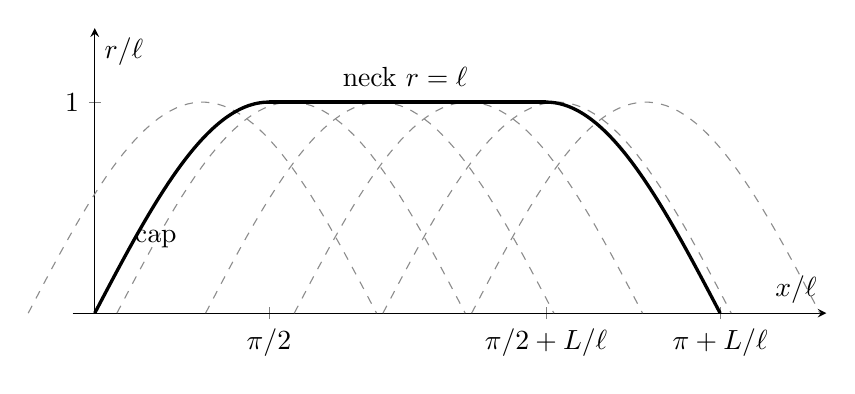
\begin{tikzpicture}
\begin{axis}[width=0.92\textwidth,height=5.2cm,axis lines=middle,xlabel={$x/\ell$},ylabel={$r/\ell$},
  xmin=-0.2,xmax=6.6,ymin=0,ymax=1.35,xtick={0,1.5708,4.0708,5.6416},
  xticklabels={$0$,$\pi/2$,$\pi/2+L/\ell$,$\pi+L/\ell$},ytick={1},clip=false]
\foreach \c in {-0.6,0.2,1.0,1.8,2.6,3.4} {
  \addplot[domain=\c:\c+3.1416,samples=60,black!45,dashed] {sin(deg(x-\c))};
}
\addplot[domain=0:1.5708,samples=60,very thick,black] {sin(deg(x))};
\addplot[domain=1.5708:4.0708,very thick,black] {1};
\addplot[domain=4.0708:5.6416,samples=60,very thick,black] {sin(deg(x-4.0708+1.5708))};
\node[black] at (axis cs:0.55,0.35) {cap};
\node[black] at (axis cs:2.8,1.12) {neck $r=\ell$};
\end{axis}
\end{tikzpicture}
\caption{The areal radius along a time-symmetric slice of the dumbbell (solid). The dashed curves are other members of the family $r=\ell\sin((x-c)/\ell)$; the neck $r=\ell$ touches every one of them at its top. It is their envelope.}
\label{fig:envelope}
\end{figure}

\section{Kinematics: what a slice looks like}

Freeze the dumbbell at a moment of time symmetry, when nothing is moving, and look at the space it occupies. Spherical symmetry lets us write its metric as
\begin{equation}\label{eq:slice}
ds^2 = dx^2 + r(x)^2\,d\Omega^2 ,
\end{equation}
where $x$ is proper distance along the axis and $4\pi r^2$ is the area of the sphere at $x$; $r$ is called the \emph{areal radius}.
The magnetic $SU(2)$ Yang--Mills field compatible with this symmetry is described by one function $W(x)$ (Chapter~12): its radial magnetic field is $(1-W^2)/r^2$ and its tangential one is $W'/r$.

Two numbers attached to each of these spheres will carry most of the argument.

\begin{definition}
The \emph{Misner--Sharp mass} of the sphere at $x$ on a time-symmetric slice is $m=\tfrac r2(1-r'^2)$.
The \emph{magnetic self-energy} of that sphere is $\ell^2(1-W^2)^2/(2r)$.
\end{definition}

For the cap $r=\ell\sin(x/\ell)$ one finds $m=\tfrac\ell2\sin^3(x/\ell)$, and for the neck $r=\ell$ one finds $m=\ell/2$.

The slice is \emph{conformally flat} when its Weyl curvature vanishes. In this sector the relevant invariant can be computed in double null coordinates, and it comes out as a difference of the two numbers above.

\begin{proposition}[Weyl curvature = mass $-$ self-energy]\proved\label{prop:weyl}
In spherically symmetric Einstein--Yang--Mills theory the conformally invariant combination of the metric functions equals
\[
3\Bigl(\frac{2m}{r}-\frac{\ell^2(1-W^2)^2}{r^2}\Bigr).
\]
Hence the slice is conformally flat exactly when $2mr=\ell^2(1-W^2)^2$: on every sphere the mass equals the magnetic self-energy.
\end{proposition}
\noindent In the repository: \lean{CFT.DS.ds\_weyl\_mass}.

\section{The action and the constraint}

The Einstein--Yang--Mills action of Chapter~13, reduced to spherical symmetry, gives one equation that every slice must satisfy, the Hamiltonian constraint. At a moment of time symmetry it reads
\begin{equation}\label{eq:ham}
-4rr''+2(1-r'^2)=4\ell^2\Bigl(W'^2+\frac{(1-W^2)^2}{2r^2}\Bigr),\qquad \ell^2=\frac{4\pi G}{g^2}.
\end{equation}
The left side is $r^2$ times the scalar curvature of the slice; the right side is $r^2$ times $16\pi G$ times the Yang--Mills energy density. You can check by hand that the cap $r=\ell\sin(x/\ell)$, $W=\cos(x/\ell)$ and the neck $r=\ell$, $W=0$ both satisfy it: in both cases the two sides are $6\sin^2(x/\ell)$ and $2$.

Multiplying \eqref{eq:ham} by $r'/4$ turns it into a statement about the mass:
\begin{equation}\label{eq:massprime}
m'=r'\,\ell^2\Bigl(W'^2+\frac{(1-W^2)^2}{2r^2}\Bigr).
\end{equation}
\noindent In the repository: \lean{CFT.DS.ds2\_mass\_prime}. The mass grows wherever the sphere grows, at a rate fixed by the energy density.

\section{A Bogomolny inequality}

Now impose conformal flatness, $2mr=\ell^2(1-W^2)^2$, and differentiate it along the slice. Using \eqref{eq:massprime} and dividing by $2\ell^2$ gives
\begin{equation}\label{eq:Q}
r r' W'^2 + 2WW'(1-W^2) + \frac{(1-W^2)^2 r'}{r}=0 .
\end{equation}
At first sight this is not illuminating. The trick, familiar from monopole physics, is to multiply by $r'$ and look for squares.

\begin{lemma}[completing the square]\proved
For all real $r\ne0$, $r'$, $W$, $W'$,
\begin{multline*}
r'\Bigl(rr'W'^2+2WW'(1-W^2)+\frac{(1-W^2)^2r'}{r}\Bigr)\\
=\frac{\bigl(rr'W'+W(1-W^2)\bigr)^2+(1-W^2)^2\,(r'^2-W^2)}{r}.
\end{multline*}
\end{lemma}

\begin{leanbox}[\texttt{ds2\_bogomolny}]
\begin{Verbatim}[fontsize=\small]
theorem ds2_bogomolny (r r' W W' : ℝ) (hr : r ≠ 0) :
    r' * (r * r' * W' ^ 2 + 2 * W * W' * (1 - W ^ 2)
          + (1 - W ^ 2) ^ 2 * r' / r)
      = ((r * r' * W' + W * (1 - W ^ 2)) ^ 2
          + (1 - W ^ 2) ^ 2 * (r' ^ 2 - W ^ 2)) / r := by
  field_simp
  ring
\end{Verbatim}
\end{leanbox}

\begin{theorem}[Bogomolny inequality for conformally flat slices]\proved\label{thm:bog}
On a time-symmetric, conformally flat slice of spherically symmetric Einstein--Yang--Mills theory, at every point where $W^2\ne1$,
\[
r'^2\le W^2 .
\]
Equality holds if and only if $W=\pm r'$, and then the slice obeys the first-order equation $rr'W'=-W(1-W^2)$.
\end{theorem}

\begin{proof}
By \eqref{eq:Q} the left side of the lemma vanishes, so the numerator on the right vanishes. It is a square plus $(1-W^2)^2(r'^2-W^2)$ with $(1-W^2)^2>0$. If $r'^2>W^2$ the numerator would be positive. At equality the second term is zero, so the square is zero.
\end{proof}
\noindent In the repository: \lean{CFT.DS.ds2\_num}, \lean{ds2\_W\_ge}, \lean{ds2\_saturated}.

\begin{remark}
Earlier chapters imposed $W=r'$ by hand, motivated by the observation that the Yang--Mills potential can be identified with the spin connection of the slice (Chapter~15). Theorem~\ref{thm:bog} shows that this condition is not an extra assumption inside the conformally flat class: it is the case of equality of an inequality that every such slice satisfies. This is the same logic as the Bogomolny bound for monopoles, where the first-order equations describe the configurations that saturate an energy inequality.
\end{remark}

\section{The circle and its envelope}

In the saturating case $W=r'$ we have $m=\tfrac r2(1-W^2)$, and conformal flatness $2mr=\ell^2(1-W^2)^2$ becomes $r^2(1-W^2)=\ell^2(1-W^2)^2$. Dividing by $1-W^2$:

\begin{theorem}[the shape equation]\proved\label{thm:circle}
On a time-symmetric, conformally flat slice with $W=r'$ and $W^2\ne1$,
\begin{equation}\label{eq:circle}
r^2+\ell^2r'^2=\ell^2 .
\end{equation}
\end{theorem}
\noindent In the repository: \lean{CFT.DS.ds\_circle\_of\_flat}.

Equation \eqref{eq:circle} says that the point $(r,\ell W)=(r,\ell r')$ moves on a circle of radius $\ell$ (\cref{fig:circle}). The cap goes round half of it, from the north pole $(0,\ell)$ through the equator $(\ell,0)$ to the south pole $(0,-\ell)$. The neck does not move at all: it sits at the single point $(\ell,0)$.

\begin{figure}[h]
\centering
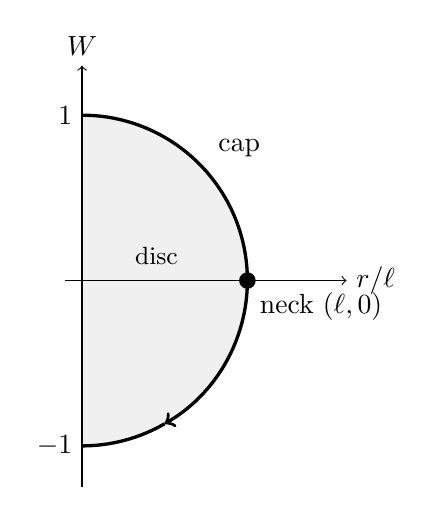
\begin{tikzpicture}[scale=2.1]
\fill[black!6] (0,-1) arc (-90:90:1) -- cycle;
\draw[->] (-0.1,0)--(1.6,0) node[right]{$r/\ell$};
\draw[->] (0,-1.25)--(0,1.3) node[above]{$W$};
\draw[very thick,black,->] (0,1) arc (90:-60:1);
\draw[very thick,black] (0.5,-0.866) arc (-60:-90:1);
\fill[black] (1,0) circle (0.05) node[below right=1pt]{neck $(\ell,0)$};
\node[black] at (0.95,0.8) {cap};
\node at (0.45,0.15) {\small disc};
\node[left] at (0,1) {$1$}; \node[left] at (0,-1) {$-1$};
\end{tikzpicture}
\caption{The $(r,W)$ plane. Conformally flat slices with $W=r'$ live on the circle $r^2+\ell^2W^2=\ell^2$. The cap runs along it; the neck is the point $(\ell,0)$. The shaded disc is the region where conformally flat solutions have real null directions (\cref{prop:disc}).}
\label{fig:circle}
\end{figure}

\begin{leanbox}[\texttt{ds\_cap\_on\_circle}]
\begin{Verbatim}[fontsize=\small]
theorem ds_cap_on_circle (l x : ℝ) :
    (l * sin (x / l)) ^ 2 + l ^ 2 * cos (x / l) ^ 2 = l ^ 2 := by
  linear_combination l ^ 2 * sin_sq_add_cos_sq (x / l)
\end{Verbatim}
\end{leanbox}

Equation \eqref{eq:circle} is of first order, and first-order equations can have solutions that are not members of the general family. Differentiating it gives $2r'(r+\ell^2r'')=0$, so at every point one of two things happens.

\begin{theorem}[two branches]\proved\label{thm:branch}
Let $r$ be twice differentiable and satisfy \eqref{eq:circle}. Then at every point
\[
r'=0\qquad\text{or}\qquad r''=-\frac{r}{\ell^2}.
\]
\end{theorem}
\noindent In the repository: \lean{CFT.DS.ds\_branch}.

The second branch is the harmonic equation; its solutions are the shifted caps $r=\ell\sin((x-c)/\ell)$, the regular solutions. The first branch, with $r^2=\ell^2$, is the constant $r=\ell$: the neck. It is the \emph{singular solution} of \eqref{eq:circle}, the envelope of the family of caps (\cref{fig:envelope}). At $r=\ell$ the equation $r'=\pm\sqrt{\ell^2-r^2}/\ell$ loses uniqueness, and this is the only place where a solution can leave the family of caps.

\begin{corollary}
A $C^1$ curve that follows a cap and then the neck must switch at a point where the cap reaches $r=\ell$. There the first derivatives agree ($r'=0$ on both sides) but the second derivatives are $-1/\ell$ and $0$. The dumbbell is $C^1$ and never $C^2$.
\end{corollary}

This is the geometric content of the ``jump'' that appeared in earlier chapters. It is not a defect put in by hand; it is the standard relation between a family of curves and its envelope: an envelope touches each curve, so slopes agree, but it does not bend with it.

\begin{proposition}[the disc]\proved\label{prop:disc}
For conformally flat solutions the slope $dW/dr$ along a null direction solves a quadratic equation with coefficients $(1-W^2)^2/r$, $2W(1-W^2)$ and $(r^2-\ell^2(1-W^2)^2)/r$. Its discriminant is
\[
\frac{4(1-W^2)^3}{r^2}\bigl(\ell^2(1-W^2)-r^2\bigr),
\]
so for $W^2<1$ real slopes exist exactly in the disc $r^2+\ell^2W^2\le\ell^2$. The two roots coincide on the circle. The whole cap spacetime, $r=\ell\cos\eta\sin\chi$ and $W=\cos\chi$, lies in the disc, since $r^2+\ell^2W^2=\ell^2-\ell^2\sin^2\eta\sin^2\chi$.
\end{proposition}
\noindent In the repository: \lean{CFT.DS.ds\_slope\_disc}, \lean{ds\_slope\_real}, \lean{ds\_cap\_disc}.

\section{Theorem A: the junction is forced}

We can now put the pieces together. Once one decides to glue a cap to a neck, nothing about the gluing is left to choose.

\begin{theorem}[uniqueness of the junction]\proved\label{thm:A}
Consider the cap $r=\ell\sin(x/\ell)$ and the neck $r=\ell$ with $W=r'$.
\begin{enumerate}[label=(\roman*)]
\item The areal radius is continuous only at the equator $x=\pi\ell/2$ (\lean{ju\_location}).
\item There $r'=\cos(x/\ell)=0$, so the first derivatives agree automatically (\lean{ju\_C1\_auto}).
\item The second derivatives are $-1/\ell$ on the cap (\lean{ju\_cap\_second}) and $0$ on the neck, and at $r=\ell$, $r'=0$ the Hamiltonian constraint \eqref{eq:ham} reduces to $r''(r''+1/\ell)=0$, whose only roots are these two values (\lean{rr\_two\_roots}).
\item The junction cannot be a timelike tube: along it the cap's equatorial radius $\sqrt{\ell^2-\tau^2}$ differs from $\ell$ for $\tau\ne0$ (\lean{rj\_tube\_mismatch}).
\item Along a null front the jump $[W_u]$ keeps its value at the corner, $1/(\sqrt2\,\ell)$ (\lean{ju\_jump\_fixed}).
\end{enumerate}
\end{theorem}
\noindent The combined statement is \lean{CFT.JU.ju\_theorem\_A}.

Part (i) surprised the author. One would expect the place of the junction to be a free choice. It is not: the largest radius of the cap is exactly the radius of the neck, so they can touch only at the top of the cap, and there the slopes agree by themselves. ``Glue continuously'' already implies ``glue in a $C^1$ way''.

\begin{standsbox}
\textbf{Known.} The cap (the closed radiation universe driven by the homogeneous Yang--Mills field) and the neck (the magnetic Bertotti--Robinson spacetime) are classical solutions \cite{Tolman,Bertotti,Robinson}. That the throat of an extremal black hole has a free length, and that it saturates an area--charge inequality, is known for Einstein--Maxwell theory \cite{DJR,CM}. The relation between the Weyl curvature and the Misner--Sharp mass is known in general \cite{MS}.

\textbf{Claimed as new, in the weak sense of the guide for the specialist.} The Bogomolny-type inequality $r'^2\le W^2$ for conformally flat slices (Theorem~\ref{thm:bog}), the reading of the neck as the singular solution and envelope of the caps (Theorems~\ref{thm:circle} and \ref{thm:branch}), and the statement that the junction is forced (Theorem~\ref{thm:A}).

\textbf{Assumptions to keep in mind.} Spherical symmetry, a purely magnetic field, time symmetry and conformal flatness. Outside the class $W=r'$ the two roots of (iii) disappear, so these theorems do not exclude a smooth interpolation in general. Inside the conformally flat class a numerical search for a smooth static interpolation failed \negative{} (Chapter~19).

\textbf{Open.} Why the dumbbell is glued at all is not answered by these theorems; they say only how it must be glued if it is. Chapter~26 shows that a fixed total volume $2\pi^2\ell^3+4\pi\ell^2L$ fixes the neck length $L$, and Chapter~23 shows that quantum mechanically $L$ is conjugate to $-r\dot r$. \open
\end{standsbox}

\section*{Exercises}
Each exercise is answered by the named Lean theorem. Read its statement in the repository and compare it with your own answer.

\begin{exercise}
Check by hand that the cap $r=\ell\sin(x/\ell)$, $W=\cos(x/\ell)$ lies on the circle \eqref{eq:circle}, and that the neck $(r,W)=(\ell,0)$ lies on it too. \emph{Answer:} \lean{ds\_cap\_on\_circle}, \lean{ds\_neck\_on\_circle}.
\end{exercise}

\begin{exercise}
Multiply the Hamiltonian constraint \eqref{eq:ham} by $r'/4$ and show that it becomes \eqref{eq:massprime}. \emph{Answer:} \lean{ds2\_mass\_prime}.
\end{exercise}

\begin{exercise}
Expand both sides of the completing-the-square lemma and check that they agree. Where is $r\ne0$ used? \emph{Answer:} \lean{ds2\_bogomolny}.
\end{exercise}

\begin{exercise}
Theorem~\ref{thm:circle} assumes $W^2\ne1$. Find what goes wrong in the proof when $W^2=1$, and describe the slices with $W\equiv\pm1$. \emph{Answer:} the division in \lean{ds\_circle\_of\_flat}; for the slices, \lean{fam\_birkhoff\_u} in Chapter~21.
\end{exercise}

\begin{exercise}
Show that $\ell\sin(x/\ell)=\ell$ with $0<x<\pi\ell$ forces $x=\pi\ell/2$. \emph{Answer:} \lean{ju\_location}.
\end{exercise}

\begin{exercise}
Compute the derivative of $\cos(x/\ell)$ at $x=\pi\ell/2$. \emph{Answer:} \lean{ju\_cap\_second}.
\end{exercise}

\begin{exercise}
Solve $2\ell^2y^2+2\ell y=0$ and explain why its two roots are the second derivatives of the neck and of the cap at the junction. \emph{Answer:} \lean{rr\_two\_roots}.
\end{exercise}

\begin{exercise}
Show that for $W^2<1$ the discriminant of \cref{prop:disc} is non-negative if and only if $r^2+\ell^2W^2\le\ell^2$. \emph{Answer:} \lean{ds\_slope\_real}.
\end{exercise}
